%%%%%%%%%%%%%%%%%%%%%%%%%%%%%%
% LATEX-TEMPLATE TECHNISCH RAPPORT
%-------------------------------------------------------------------------------
% Voor informatie over het technisch rapport, zie
% http://practicumav.nl/onderzoeken/rapport.html
% Voor readme en meest recente versie van het template, zie
% https://gitlab-fnwi.uva.nl/informatica/LaTeX-template.git
%%%%%%%%%%%%%%%%%%%%%%%%%%%%%%

%-------------------------------------------------------------------------------
%	PACKAGES EN DOCUMENT CONFIGURATIE
%-------------------------------------------------------------------------------

\documentclass{uva-inf-article}
\usepackage[english]{babel}
\usepackage[table,xcdraw]{xcolor}
\usepackage{float}
\usepackage{graphics}
\usepackage{pdfpages} 


% Relevant voor refereren vanaf blok 5
\usepackage{cite}
\usepackage[style=authoryear-comp]{biblatex}
\addbibresource{Project/ProjectPlan/LaTeX/main.bib}

%-------------------------------------------------------------------------------
%	GEGEVENS VOOR IN DE TITEL
%-------------------------------------------------------------------------------

% Vul de naam van de opdracht in.
\assignment{Graduation project Bacheler of Computer Science}
% Vul het soort opdracht in.
\assignmenttype{Project plan}
% Vul de titel van de eindopdracht in.
\title{Development of an interactive experiment on the effect of sequential information on the formation of generic beliefs}

% Vul de volledige namen van alle auteurs in.
\authors{Bodi Boelé}

% Vul de corresponderende UvAnetID's in.
\uvanetids{11904089}

% Vul altijd de naam in van diegene die het nakijkt, tutor of docent.
\tutor{Dr. Patricia Mirabile}
% Vul eventueel ook de naam van de docent of vakcoordinator toe.
\docent{dhr. dr. R.G. (Rob) Belleman}
% Vul hier de naam van de PAV-groep  in.
\group{}
% Vul de naam van de cursus in.
\course{Afstudeerproject bachelor Informatica}
% Te vinden op onder andere Datanose.
\courseid{5062ABI18Y}

% Dit is de datum die op het document komt te staan. Standaard is dat vandaag.
\date{\today}

%-------------------------------------------------------------------------------
%	VOORPAGINA
%-------------------------------------------------------------------------------

\begin{document}
\maketitle

%-------------------------------------------------------------------------------
%	Inhoudsopgave
%-------------------------------------------------------------------------------
%-------------------------------------------------------------------------------
%	Achtergrond
%-------------------------------------------------------------------------------

\section{Background}
`Ducks lay eggs', `tigers are striped', `lions have manes' and `ticks spread Lyme disease'. These are all generic statements. Generics statements express generalizations about the members of a kind. The statements mentioned lack any form of quantification and are therefore `bare'. 

`Bare' generic statements express useful generalizations, but it is difficult to come to an unambiguous conclusion on when people think these statements are true. There is no unique critical point where people in general tend to designate a statement as true. For example when people have to judge the statement `lions have manes', the predominant conclusion will be true, although less than 50\% of lions (only the older male lions) have manes. When asked about the statement `ticks spread Lyme disease' the predominant conclusion as well would be true, even though the statement is only true for 2.7\% \parencite{rivm_2019} of tick bites that actually transfer the disease whereas 20\% of ticks carry the disease. These rather large differences in truth-conditions are described in \cite{leslie2011all}. 

The research by \cite{leslie2011all} conducts an experiment in which they compare how people assert different formulations of generic statements. People have the opportunity to indicate whether they agree with one of the items on a 6 point scale. Even when people are given correct alternatives (e.g. `male lions have manes' and `lions have manes') people overgeneralize and agree more with the `false'\footnote{There is no true or false, but people tend to choose the over generalized (less true) item over the more defined item.} item.  

\newpage
%-------------------------------------------------------------------------------
%	Projectdoelstelling
%-------------------------------------------------------------------------------
\section{Relevant readings}
Research on the topic of generic statements has been part of the field of scientific research for quite a while. Experimental psychology as well as philosophy of language have been doing research on generic statements for quite a while now. 

Experimental psychology has highlighted a number of biases and preferences such as the generic overgeneralization effect, the bias for people to accept a generic statement based on rare events and the biased position of people where they are more negatively biased towards non-human categories. For example people tend to classify `Men attack people' as false and `Sharks attack people' as true, even though the chance of men attacking people is vastly higher than the chance of sharks attacking people. 

The generic overgeneralization effect, as described by \cite{leslie2011all}, shows that people tend to falsely accept (over)generalized statements when offered a more descriptive alternative, as described in the previous section. 

Another relevant research project in the domain of experimental psychology is the project by \cite{tasimi2017differences} which concludes that people are biased towards generics involving non-human entities. Their research also suggests that it is necessary expand on the cognitive processes underlying these effects which is part of the goal of the overarching research project of this project.

\cite{cimpian2010generic} states that `generic statements require little evidence for acceptance' such as the previously mentioned tick example and other striking generics like `Rottweilers maul children' and `Lions eat people' even though these statements are only true for exceptional cases. According to their research generic statements are often judged true based on little evidence, but these implications go far beyond what is needed to accept them. This underlines the importance of the parent research on how people form these beliefs and what the effect of sequential information is on their judgment. \\

Within the field of philosophy of language the study performed by \cite{van2020generics} analysed generic statements based on the intuition that other authors, over the years, claimed to be natural. In their paper they suggest that people tend to accept and interpret generics based on a distorted picture of it provided by the media instead of on actual frequencies.

%-------------------------------------------------------------------------------
%	Projectresultaat
%-------------------------------------------------------------------------------
\section{Research question}
The goal of this project is to create software which will be used for a scientific research project on the effect of sequential information on the formation of generic beliefs. The project seeks to approximate learning on the basis of iterative information. The program therefore needs an interactive interface which allows to scale the experiment depending on the users answers. The end product will be an online experiment where participants are able to interact with the environment, discover information about the objects inside it and evaluate generic statements about those objects. 

The final result of this thesis will be the online hosted experiment that can be used for the aforementioned scientific research project. The results gathered with this tool during the pilot experiment will be published in a final thesis, along with a short analysis, the source code and the necessary documentation.

This research project will be about creating software and therefore the research question and therefore be more focused on the software than on the underlying experiment: `How to develop an interactive online experiment that will help investigate how people acquire generic beliefs from information they learn in a sequential fashion?'
Throughout the project challenges will be encountered and therefore this thesis will also focus on these challenges: `What are the challenges to developing software that can be used for experiments in language cognition?'


%-------------------------------------------------------------------------------
%	Projectorganisatie
%-------------------------------------------------------------------------------
\section{Organisation}
\subsection{Method}
The project will be a combination of a literature review, setting up the experiment's environment, executing a pilot experiment and submitting this instrument to be used in a bigger scale research project, by hosting it online.
\subsubsection{Communication}
\begin{itemize}
    \item Zoom - Planned meetings through Zoom, every Wednesday at 4pm.
    \item Email - For questions outside the Zoom meetings.
    \item Logbook - Keep track of progress made, available on GitHub
    \item Github - Keep track of coding and progress being made, as keeping files available at all times.
\end{itemize}

%-------------------------------------------------------------------------------
%	Projectplanning
%-------------------------------------------------------------------------------
\section{Planning}
The table below shows a graphical display of the proposed deadlines for the project.
\begin{table}[H]
\centering
\caption{Deadlines}
\label{my-label}
\begin{tabular}{cp{1cm}p{5cm}p{5cm}}
Date & Type & Assignment & Necessities  \\
\hline
April 2nd (23h59) & Personal & Project plan & Send to supervisor for approval \\
April 3rd (23h59) & Project & Project plan & Approval by project supervisor \\
April 24 (23h59) & Personal & First draft of the thesis & Send to supervisor for approval \\
May 1st (23h59) & Project & First draft of the thesis & Layout (Better if first chapter finished and sections of the other chapters have been set up)\\
May 29th (23h59) & Personal & `Go'/`no-go' version of the thesis & Send to supervisor for approval \\
June 5th (23h59) & Project & `Go'/`no-go' version of the thesis & Approval by project supervisor \\
June 15th (23h59) & Project & Final version of the thesis & Approval by project supervisor \\
June 15th (23h59) & Project & Delta document of the thesis & Briefly indicate the changes that have been made compared to the Go / No-go version of the thesis.
\end{tabular}
\end{table}

These deadlines can be used as a guide for the critical points of the project. Intermediate critical points have to be formed during the project itself. These intermediate points depend on the design and how this affects the overall flow of the project. Some critical points, such as that results must be in by the end of May. It is also important that the workload of the thesis itself is spread out throughout the project instead of postponing this till the very end. 
In conclusion, there is one extremely critical dependence which is the correct functioning of the code/software.

\subsection{GanttProject}
The GanttProject planning in figure \ref{fig:planning} has been included to be used as a guideline. (A full-page version has been added as Appendix 6.1)
\begin{figure}[H]
 \centering
 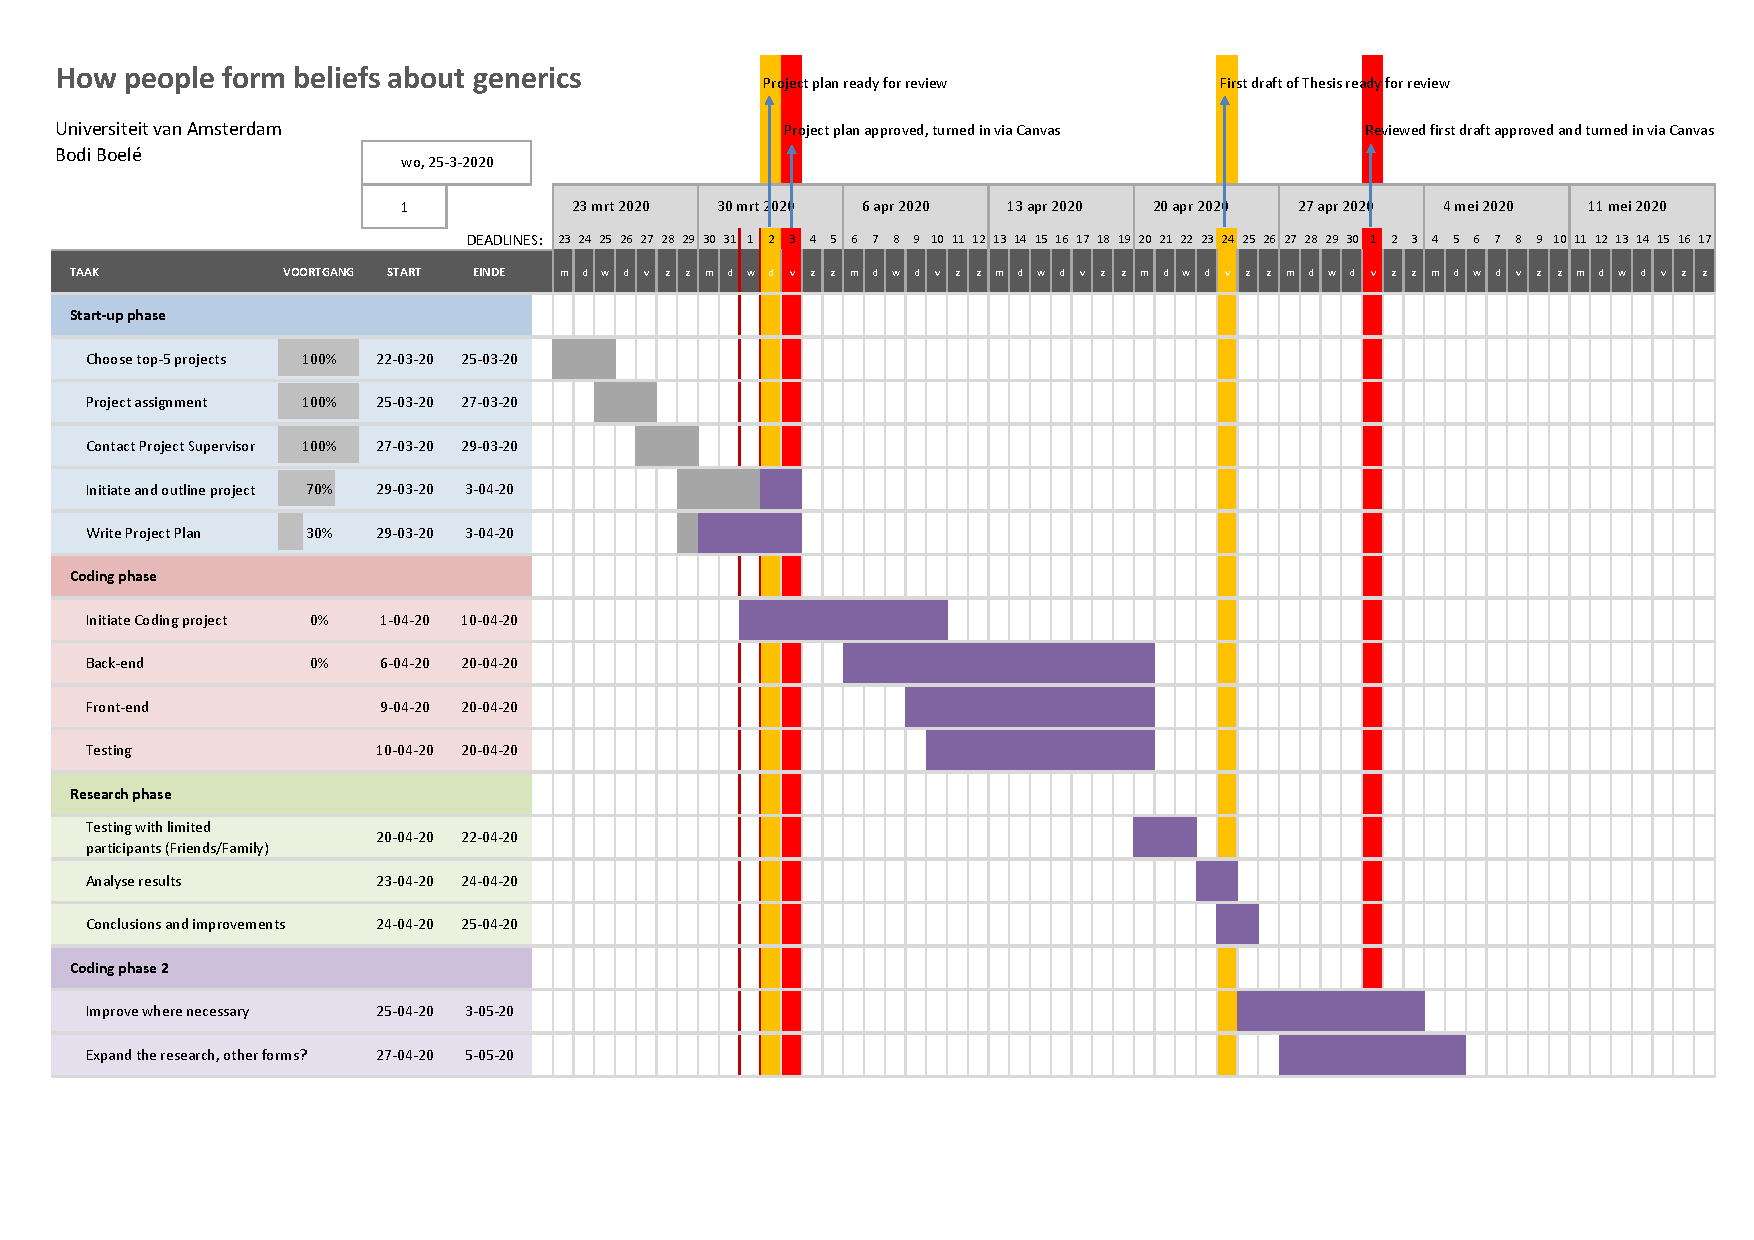
\includegraphics[page=1,width=1.1\textwidth]{Project/ProjectPlan/Gant_planning_Afstudeerproject.pdf}
 \caption{GanttProject planning (d.d. 1-4)}
 \label{fig:planning}
\end{figure}

\printbibliography

\section{Appendix}
\subsection{GanttProject.pdf}
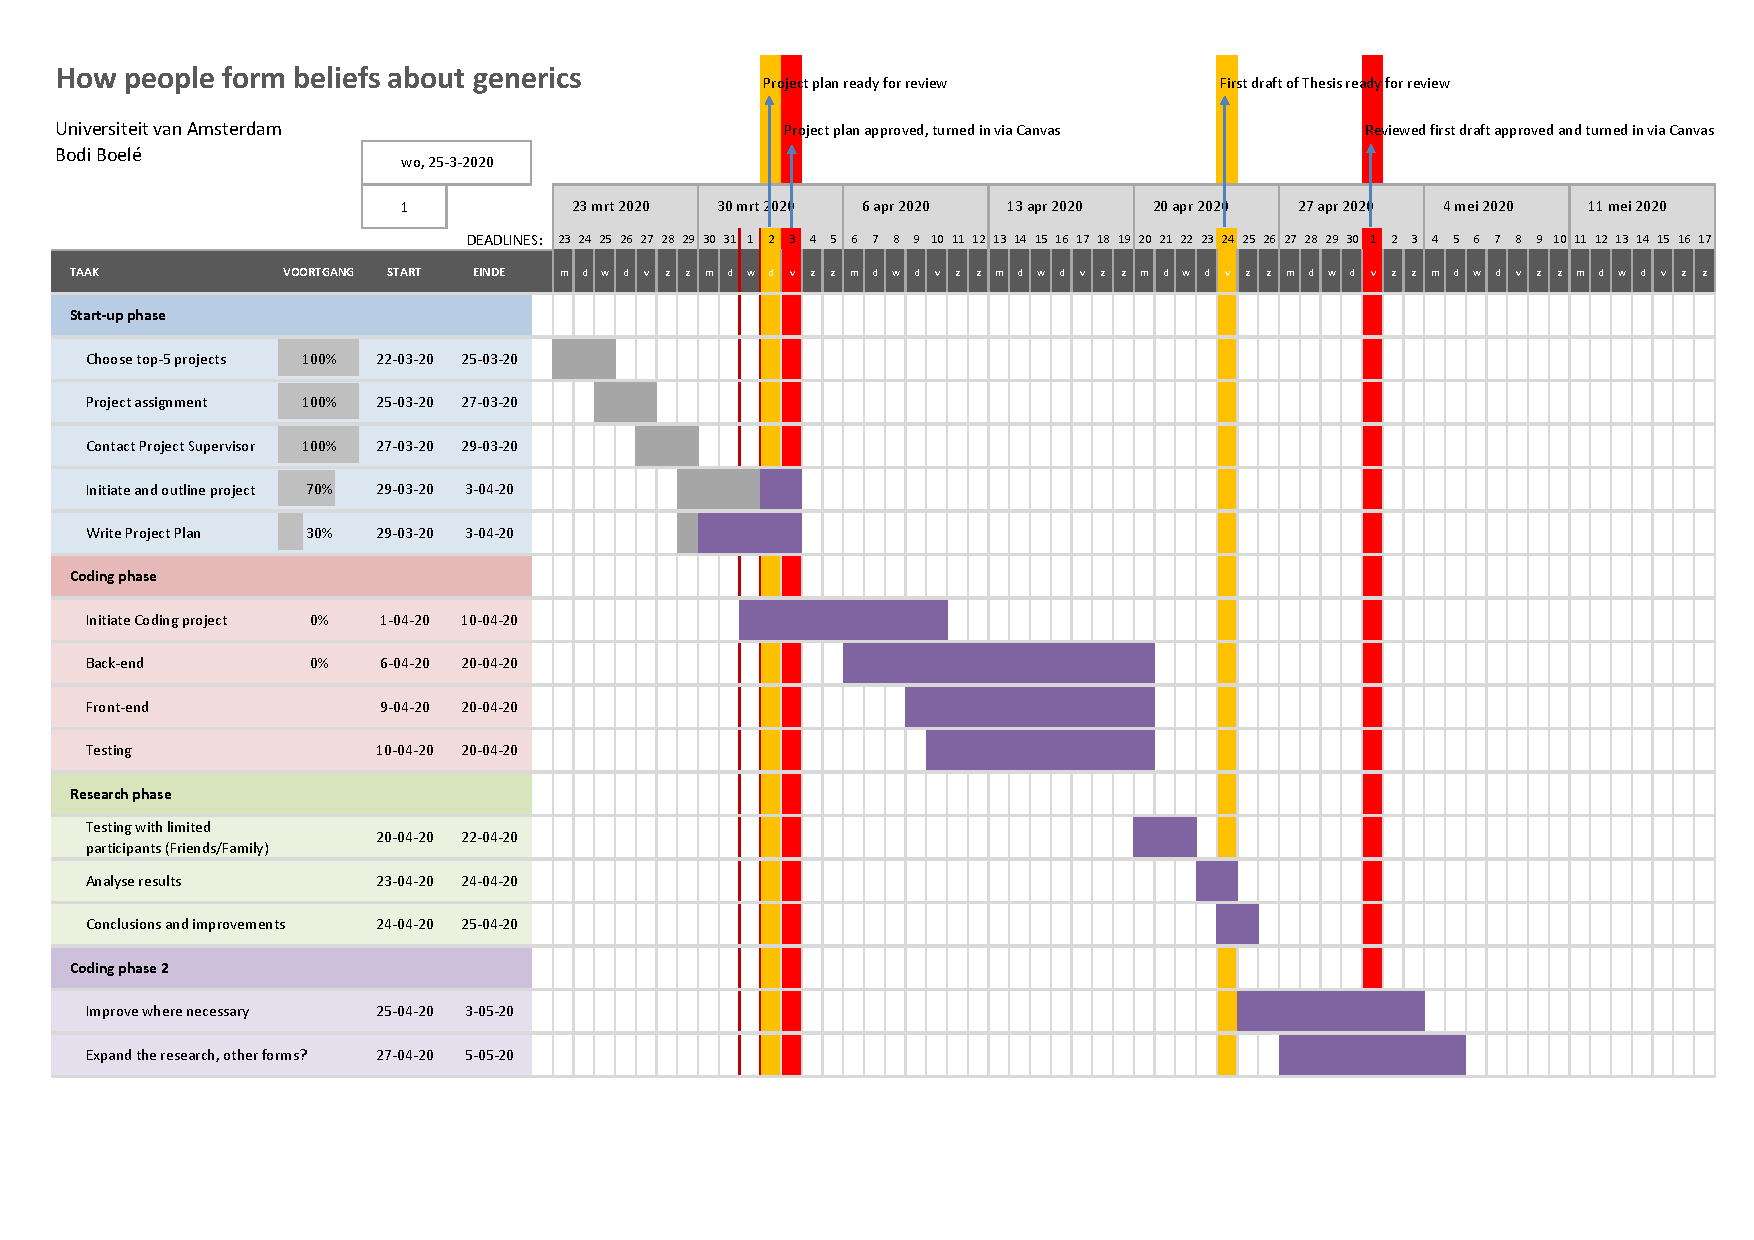
\includepdf[angle=-90, pages=-]{Project/ProjectPlan/Gant_planning_Afstudeerproject}
%-------------------------------------------------------------------------------
%	EINDE
%-------------------------------------------------------------------------------
\end{document}
